% !TeX spellcheck = en_GB
\section{Simulations Experiments}
\subsection{Study on Response Time Limits}
Before choosing the extremes of the \textbf{mean inter-arrival time} factor, a study on the \textbf{mean response time}, by changing the latter, has been carried out by comparing limit values of other factors (all the ranges will be shown in the next section).  
 \begin{figure}[H]
 	\centering
 	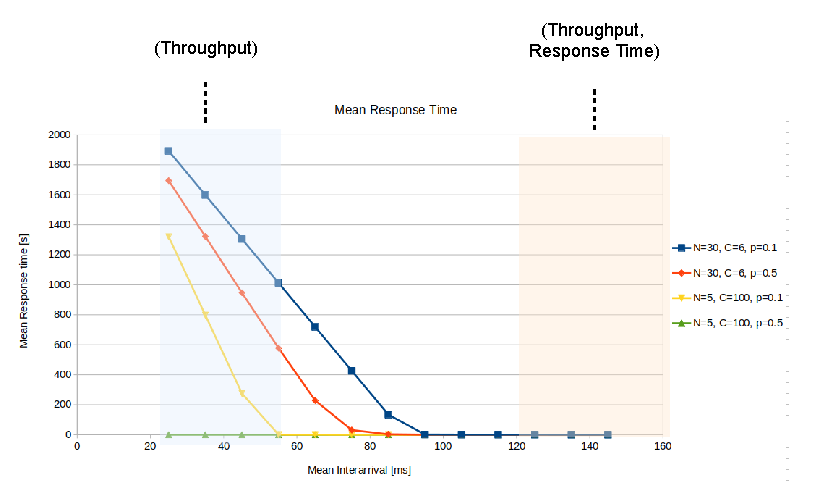
\includegraphics[width=\textwidth]{img/BufferExplosion.pdf}
 	\caption{Response Time Behaviour changing the Mean Inter-arrival Time}
 	\label {img: warmUp}
 \end{figure}
\noindent Basically, two different zone of interest of the mean inter-arrival time were found: 
\begin{itemize}
	\item the first one between \textbf{[25ms, 55ms]}, for which the mean response time diverges for the majority of the combination of other factors limits. In this area \textbf{only information about the throughput} can be carried out, because the \textbf{mean response time}, as diverges, is \textbf{dependent on the simulation duration}.
	\item the second one between \textbf{[125ms, 500ms]}, for which both information about the \textbf{throughput} and the \textbf{response time} can be carried out.
	
\end{itemize}

For the second interval, the left bound was chosen when the mean-response time began to be comparable with the time-slot duration (which will be 5ms) and the 95\% CI scissor is small in comparison with the scale of the response time (basically when the standard deviation becomes very small). Here a "zoom" on the rightmost part of the latter plot:
\begin{figure}[H]
	\centering
	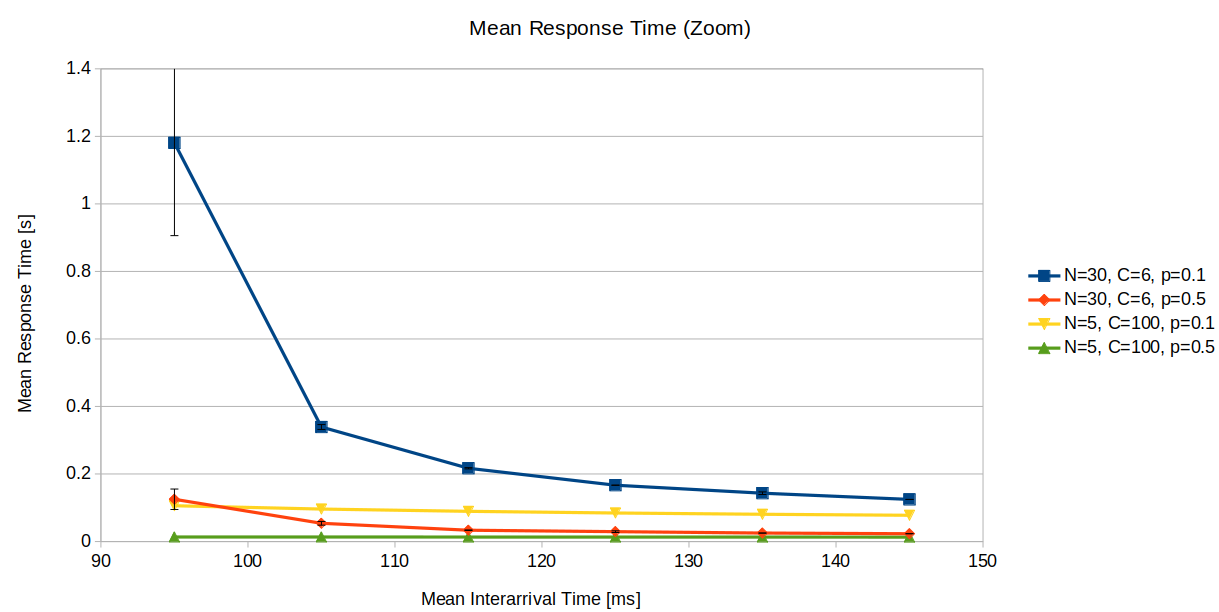
\includegraphics[width=\textwidth]{img/BufferExplosionZoom.png}
	\caption{Buffer Explosion between 95ms and 145ms: the 95\% CI are too small to be seen on the right part of the plot}
	\label {img: bufferExplosion}
\end{figure}

\subsection{Scenario Calibration}
In order to calibrate the simulator parameters, the following range of values were used:

\paragraph{Limited Response Time Scenario}
\begin{itemize}
	\item \textbf{Number of Couples Tx-Rx (N)}: [5, 30]
	\item \textbf{Number of Channels (C)} : [6, 100] (Resource Blocks in LTE for different Frequencies)
	\item \textbf{Mean Inter-arrival Time ($\frac{1}{\lambda}$)}: [125ms, 500ms]  
	\item \textbf{Time-slot duration ($T_{slot}$)}: 5 ms
	\item \textbf{Send Probability (p)}: [0.1, 0.5] 
\end{itemize}

\paragraph{Explosion of Response Time Scenario}
\begin{itemize}
	\item \textbf{Number of Couples Tx-Rx (N)}: [5, 30]
	\item \textbf{Number of Channels (C)} : [6, 100]
	\item \textbf{Mean Inter-arrival Time ($\frac{1}{\lambda}$)}: [25ms, 55ms] 
	\item \textbf{Time-slot duration ($T_{slot}$)}: 5 ms
	\item \textbf{Send Probability (p)}: [0.1, 1] 
\end{itemize}
\subsection{Calibration of Warm-Up Period and Simulation duration}
For calibrating the warm-up different simulation were made (with the factors range in the latter paragraph). After various test we found that the KPI that impacts heavily in the choose of the warmup time is the \textit{Response Time}.\\
The worst case in terms of convergence time was encountered with \textbf{N = 30, C = 6, $\dfrac{1}{\lambda}$ = 125ms, p = 0.1 }
%The worst case in terms of convergence time was encountered with the \textbf{mean throughput} with N = 5, C = 6, $\dfrac{1}{\lambda}$ = 500ms, p = 0.5:
\begin{figure}[H]
	\centering
	\includegraphics[width=\textwidth]{img/warmup.png}
	\caption{Worst Case Warm-up Response Time}
	\label {img: warmUp}
\end{figure}  
%With the \textbf{mean response time} the worst case is the following with N = 5, C = 100, $\dfrac{1}{\lambda}$ = 25ms, p = 0.5:

\noindent\textbf{A warm-up period of 250s was chosen}.\\
For what concerns the simulation duration was made a trade-off between the \textbf{memory and time consumption} for storing data and performing simulation and the tendency of the KPIs to achieve a \textbf{more stable standard deviation}. This was done because there are not stochastic elements in the model (like a particular error probability with a low percentage) that will need a particular amount of time to be shown. Obviously the duration has to be greater than the warm-up duration. All things considered, \textbf{a simulation-duration of 5000s was chosen}.

\subsection{Limited Response Time Scenario Study}
In this chapter we will enter more in the deep to the limited response time scenario, in order to find insights about \textbf{throughput} and \textbf{response time} (we can due to the fact that in this interval it converges).
\subsubsection{Factorial Analysis $2^kr$ on Throughput}
In order to analyse the contribution of the factors on the throughput performance, we perform a $2^kr$ analysis with $r=5$ and $k=4$ (so we perform $5\cdot2^4 = 80$ experiments). We take into account the following factors:
\begin{itemize}
	\item Number of Couples Tx-Rx (\textbf{N}): [5, 30] \textbf{(A)}
	\item Number of Channels (\textbf{C}) : [6, 100] \textbf{(B)}
	\item Send Probability (\textbf{p}): [0.1, 0.5] \textbf{(C)}
	\item Mean Inter-arrival Time ($\dfrac{1}{\lambda}$): [125ms, 500ms] \textbf{(D)}    
\end{itemize}

\noindent The first step is to \textbf{check the hypothesis}, in particular we have to control that the \textbf{residuals are normal} and that its \textbf{standard deviation is constant} (a.k.a. homoskedasticity). For what concerns the normal hypothesis it's possible to see (Figure \ref{img: qqplot_throughput}) that the QQ plot of residuals vs normal \textbf{show a linear tendency} and so the \textbf{hypothesis is verified}.

\noindent For the\textbf{homoskedasticity}, we have a QQ plot residuals vs predicted response and we can see (Figure \ref{img: homoskedasticity_throughput}) that indeed there is a trend, however the \textbf{errors} (y axis) \textbf{are two order of magnitude below the predicted response} (x axis) and so \textbf{we can ignore trends} and state that the \textbf{homoskedasticity hypothesis is respected}.

\begin{figure}[H]
	\centering
	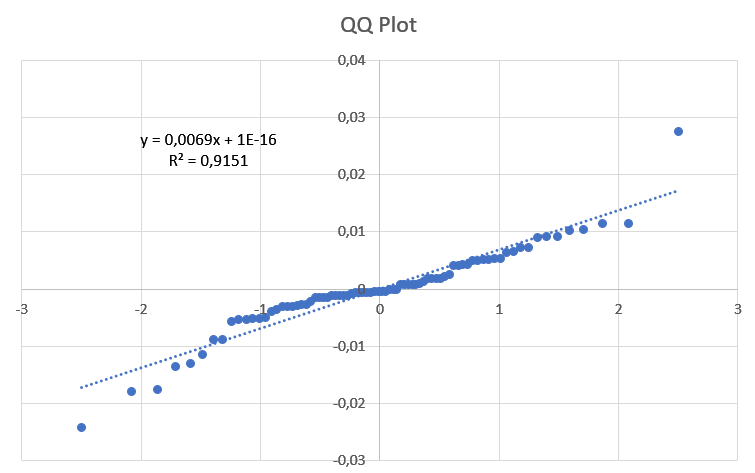
\includegraphics[width=0.85\textwidth]{img/QQplot_2kr_throughput.png}
	\caption{QQ Plot for testing the normal hypothesis}
	\label {img: qqplot_throughput}
\end{figure}

\begin{figure}[H]
	\centering
	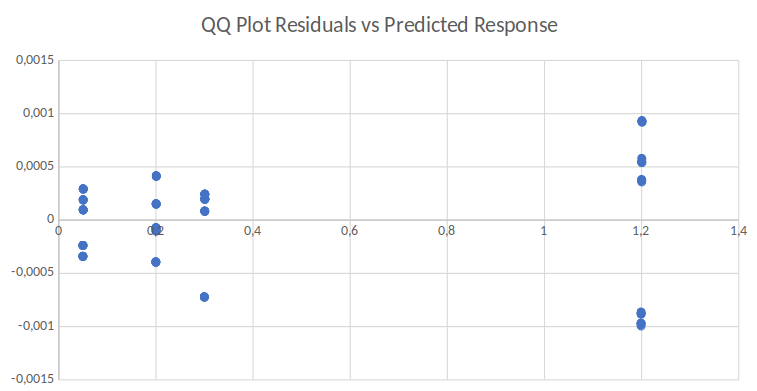
\includegraphics[width=0.85\textwidth]{img/homoskedasticity_2kr_throughput.png}
	\caption{QQ Plot for testing homoskedasticity}
	\label {img: homoskedasticity_throughput}
\end{figure}

\noindent Now we can analyse the obtained results. The most relevant ones are the one in the following list, the other factors have an impact on the variability that is very low, ($<<1\%$) and so they are non relevant:

\begin{itemize}
	\item \textbf{Number of Couples (N)}
	
	\noindent It has a \textbf{positive impact} on throughput, in particular $qi = [0,312532; 0,312537]$\footnote{This and the following are 95\% confidence interval} and it accounts for the \textbf{48,44\%} of the variability. This means that the \textbf{higher the number of couples the higher the throughput}. In fact with more transmitters we have more packets and so we have an higher throughput.
	 
	\item \textbf{Mean Inter-Arrival Time ($\dfrac{1}{\lambda}$)}
	
	\noindent It has a \textbf{negative impact}: $qi = [-0,262444; -0,262439]$ and it accounts for the \textbf{34,15\%} of the variability. Thus we can say that the \textbf{higher the mean inter-arrival time, the lower the throughput}. This happens due to the fact that when we increase the mean inter-arrival time it's more likely that a transmitter have an empty buffer and so it has no packets to transmit, then the throughput decreases. 
	
	\item \textbf{Jointly Effect of Number of Couples and Mean Inter-Arrival Time}
	
	\noindent The \textbf{jointly effect of the above factors} accounts for the \textbf{17,39\%} of the variability and it has a \textbf{negative impact} ($qi = [-0,187301; -0,187296]$). This because the \textbf{effect of the mean inter-arrival time is greater with respect to the one of the number of couples}, so \textbf{if both increase then the throughput decreases}. Indeed, if we have an higher number of transmitters, but we have the most of them which have an empty buffer (due to the previously explained phenomenon caused by the increasing of the mean inter-arrival time), then the throughput decreases because there are too few packets to transmit.
\end{itemize}

\subsubsection{Factorial Analysis $2^kr$ on Response Time}
Now let analyse the contribution of factors on the other KPI, the \textbf{Response Time}. Also in this case, as the previously, we perform a $2^kr$ analysis with $r=5$ and $k=4$ and so 80 experiments in total. The factors are the same of the previously analysis.

\noindent %\colorbox{yellow}{We can see the plots to check} the hypothesis in figure \ref{img: qqplot_responsetime} (for what concerns the normal hp) and in figure \ref{img: homoskedasticity_responsetime} (for what concerns the homoskedasticity).

%\begin{figure}[H]
%	\centering
%	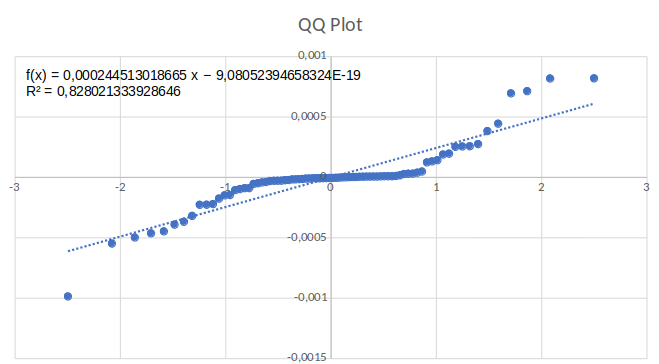
\includegraphics[width=0.8\textwidth]{img/qqplot_2kr_responsetime.png}
%	\caption{\colorbox{yellow}{QQ Plot for testing} the normal hypothesis}
%	\label {img: qqplot_responsetime}
%\end{figure}

%\begin{figure}[H]
%	\centering
%	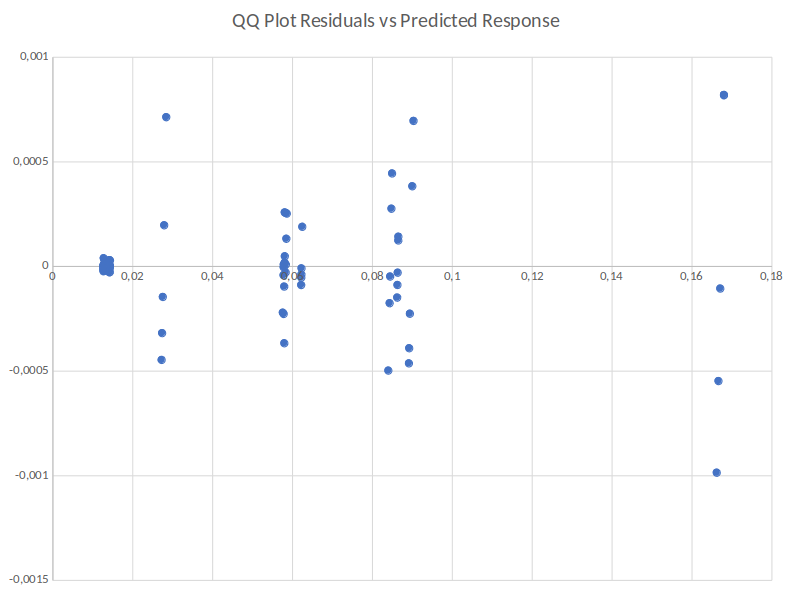
\includegraphics[width=0.8\textwidth]{img/homoskedasticity_2kr_responsetime.png}
%	\caption{\colorbox{yellow}{QQ Plot for testing} homoskedasticity}
%	\label {img: homoskedasticity_responsetime}
%\end{figure}

%\noindent \colorbox{yellow}{The plot about the normal hp} is obtained through a logarithmic transformation and it shows an approximating linear trend. Instead for the homoskedasticity we can see that there is a trend but the errors are at least one order of magnitude below the predicted response, and so also this hypothesis is verified.

\noindent After verifying the hypothesis as shown in the in the latter section, the most relevant contributions are the ones explained in the following lists, the others one have an impact in the variability that is negligible w.r.t. the following ones: 

\begin{itemize}
	\item \textbf{Send Probability p}
	
	\noindent It has a \textbf{negative impact} on the response time, in particular $qi = [-0,033928; -0,033926]$ and it accounts for the \textbf{65,67\%} of the variability. This means that the \textbf{higher the send probability the lower the response time}. In fact with an high send probability it's more likely that a packet will sent (both in the case of first transmission and in the case of retransmission because of collision) and so it doesn't remain in the transmitter queue increasing its response.  
	
	\item \textbf{Mean Inter-Arrival Time}
	
	\noindent It has a \textbf{negative impact}: $qi = [-0,012955; -0,012954]$ and it accounts for the \textbf{9,57\%} of the variability. Thus we can say that the \textbf{higher the mean inter-arrival time, the lower the response time}. This happens due to the fact that when we increase the mean inter-arrival time it's more likely that transmitters send few packets in a slot time and so the probability of having collisions, and so the necessity of retransmitting a packet, is lesser. Moreover even if a collision occurs with an higher mean inter-arrival time there are not several packets in the transmitter queue and so the response time decreases. 
\end{itemize}

\newpage
\subsubsection{$2^kr$ Overall Results}
As a reference, in the table \ref{tab: 2kr_results} we can see the results obtained through the $r2^k$ analysis.
\begin{itemize}
	\item Number of Couples Tx-Rx: [5, 30] \textbf{(A)}
	\item Number of Channels C : [6, 100] \textbf{(B)}
	\item Send Probability p: [0.1, 0.5] \textbf{(C)}
	\item Mean Inter-arrival Time: [125ms, 500ms] \textbf{(D)}    
\end{itemize}
\begin{table}[H]
	\centering
	\begin{tabular}{|c|c|c|c|c|}
		\hline
		\textbf{} & \multicolumn{2}{c|}{\textit{\textbf{Throughput}}} & \multicolumn{2}{c|}{\textit{\textbf{Response Time}}} \\ \hline
		Factors   & qi          & Impact on Variability (\%)          & qi            & Impact on Variability (\%)           \\ \hline
		A    & 0,312534      & 48,44\%    & 0,006183  & 2,18\%  \\ \hline
		B    & -4,342100 x $10^-7$ & 9,35 x $10^{-11}$\% & -0,006719 & 2,57\%  \\ \hline
		C    & -6,710519 x $10^-7$ & 2,23 x $10^{-10}$\% & -0,033927 & 65,67\% \\ \hline
		D    & -0,262442     & 34,15\%    & -0,012954 & 9,57\%  \\ \hline
		AB   & -1,447366 x $10^-7$ & 1,03 x $10^{-11}$\% & -0,005873 & 1,96\%  \\ \hline
		AC   & -9,078937 x $10^-7$ & 4,08 x $10^{-10}$\% & -0,004269 & 1,04\%  \\ \hline
		AD   & -0,187298     & 17,39\%    & -0,005481 & 1,71\%  \\ \hline
		BC   & 5,657888 x $10^-7$  & 1,58 x $10^{-10}$\% & 0,004619  & 1,21\%  \\ \hline
		BD   & 4,342100 x $10^-7$  & 9,35 x $10^{-11}$\% & 0,005906  & 1,99\%  \\ \hline
		CD   & 1,973682 x $10^-7$  & 1,93 x $10^{-11}$\% & 0,010951  & 6,84\%  \\ \hline
		ABC  & 4,868415 x $10^-7$  & 1,17 x $10^{-10}$\% & 0,004054  & 0,93\%  \\ \hline
		ABD  & 1,447366 x $10^-7$  & 1,03 x $10^{-11}$\% & 0,005238  & 1,56\%  \\ \hline
		ACD  & 8,552622 x $10^-7$  & 3,62 x $10^{-10}$\% & 0,003929  & 0,88\%  \\ \hline
		BCD  & -6,710519 x $10^-7$ & 2,23 x $10^{-10}$\% & -0,004240 & 1,02\%  \\ \hline
		ABCD & -4,868415 x $10^-7$ & 1,17 x $10^{-10}$\% & -0,003761 & 0,80\%  \\ \hline
	\end{tabular}
	\caption{Results of $r2^k$ analysis for Throughput and for Response Time. 95\% of confidence.}
	\label{tab: 2kr_results}
\end{table}
																
\subsection{Limited Response Time Scenario: Result Analysis}
Our objective is (as we said at the beginning of the report) the \textit{Assessment of the Effectiveness of the Slotted Random-Access Network Protocol}. In order to do so we choose the mean response time and the mean throughput as Key Performance Indexes. For each KPI we set 2 scenarios: one for \textbf{low traffic condition} (in terms of Transmitters and Channels) and the other one for \textbf{high traffic condition}. For each factor variation of each scenario of each KPI we perform 35 repetitions in order to obtain meaningful and statistically valid data. Data are computed with a confidence level of 95\% (to small to be seen). Thanks to the analysis performed on this two scenarios and studying the evolution of the KPIs in them, we are able to reach our aim and give some insights on the network protocol. 

\subsubsection{Throughput}
For what concerns the throughput we set these two scenarios:
\begin{enumerate}
	\item \textit{High Traffic Scenario}
	
	N = 30, C = 6, Send Probability = 0.1
	\item \textit{Low Traffic Scenario}
	
	N = 5, C = 100, Send Probability = 0.1
\end{enumerate}

\noindent In both scenarios we \textbf{vary the mean inter-arrival time} from 125 ms to 500 ms with a step of 75 ms. In fact as we seen in the $2^kr$ analysis it is the most relevant factor for the throughput. 

\noindent We can see the results obtained in the outlined scenarios when the mean inter-arrival time grows from 125 ms to 500 ms in figure \ref{img: insight1_throughput}.

\begin{figure}[H]
	\centering
	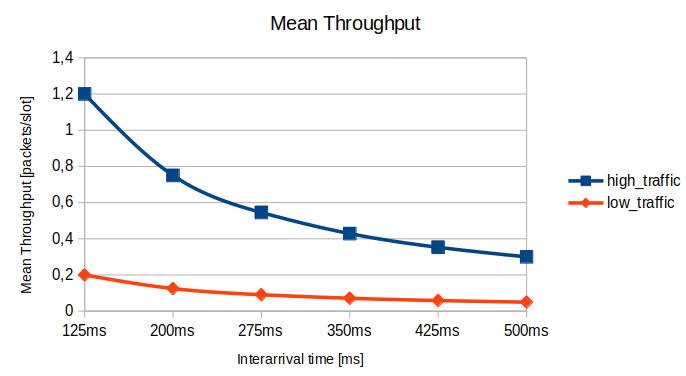
\includegraphics[width=0.9\textwidth]{img/insight1_throughput.png}
	\caption{Insight 1}
	\label{img: insight1_throughput}
\end{figure}

\noindent From the plot we can state that the \textbf{throughput is higher in the high traffic scenario}, because the more the traffic the more the packets. We can also see that the \textbf{best results is obtained with the lower mean inter-arrival time}, this because we have to consider the time slot duration that is 5 ms and it is a lot smaller than the mean inter-arrival time: if the mean inter-arrival time increases, then there are slots where no packets are transmitted (because transmitters have no packets in the queue) and this affect the mean throughput and this is the reason why the throughput decreases with the increase of the mean inter-arrival time. So the latter is another validation of what we obtain from the $2^kr$ analysis. So at the end we can say that the \textbf{throughput depends mainly from the traffic and from the mean inter-arrival time}, this is good because this means that the effect of collisions doesn't not affect so much the overall performance of the network protocol with this particular scenario. In fact in the high traffic condition there are more collisions w.r.t. to the scenario with low traffic, but nevertheless the throughput it is not affected by this.

%\noindent \colorbox{yellow}{Now let analyse the fairness} of the network protocol for what regards the throughput. It's possible to see the Lorenz Curve for both scenarios in figure \ref{img: insight2_throughput}, we show one figure for both cases because they are indeed equals.

%\begin{figure}[H]
%	\centering
%	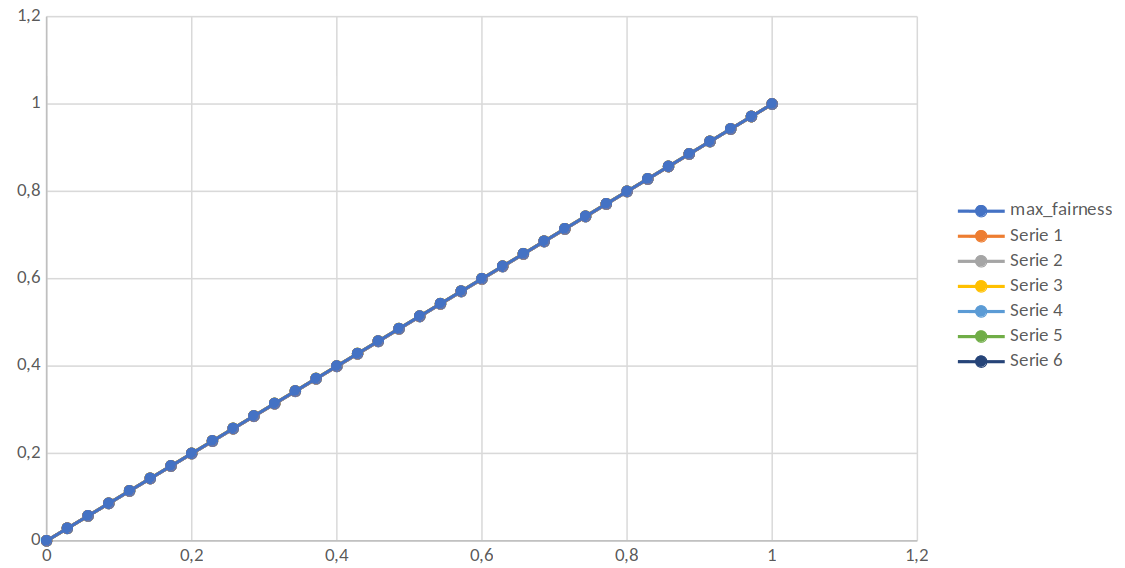
\includegraphics[width=0.7\textwidth]{img/lorenz_throughput.png}
%	\caption{\colorbox{yellow}{Insight 2}}
%	\label{img: insight2_throughput}
%\end{figure}

%\noindent \colorbox{yellow}{As we can see in the plot in all cases} the network protocol is fair for what regards the throughput.

\subsubsection{Response Time}
For what concerns the response time we set these two scenarios:
\begin{enumerate}
	\item \textit{High Traffic Scenario}
	
	N = 30, C = 6, Mean Inter-Arrival Time = 125 ms
	\item \textit{Low Traffic Scenario}
	
	N = 5, C = 100, Mean Inter-Arrival Time = 125 ms
\end{enumerate}

\noindent In both scenarios we \textbf{vary the send probability} from 0.1 to 1 with a step of 0.1, in fact for the response time the latter is the most relevant factor (as we seen in the $2^kr$ analysis) and so it is the only that if changes causes a big difference.

\noindent The results obtained in the previously explained scenario when the send probability (p) varies from 0.1 to 1 is shown in figure \ref{img: insight1_respTime}.
\begin{figure}[H]
	\centering
	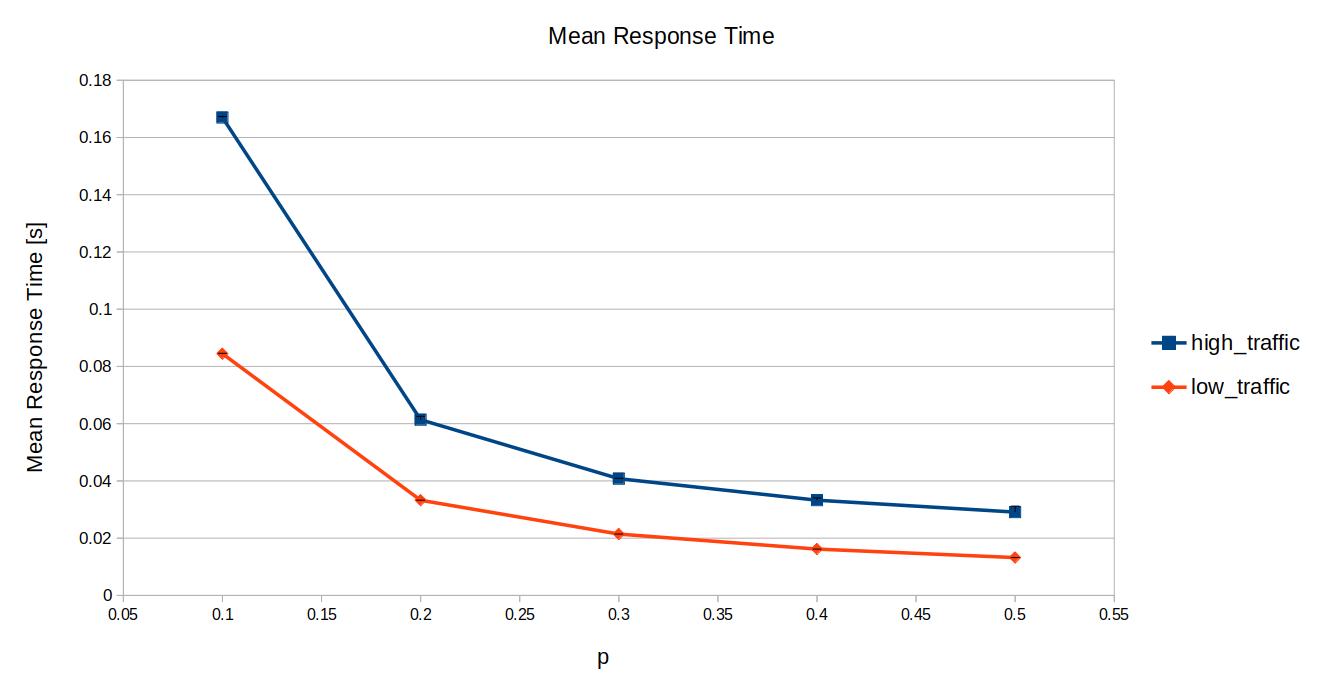
\includegraphics[width=\textwidth]{img/MeanResponseTimeInsight.png}
	\caption{Insight 1}
	\label{img: insight1_respTime}
\end{figure}

\noindent From the figure we can infer that in the \textbf{high traffic scenario the response time is higher} than the low traffic scenario, this is something normal. Then we can also say that the m\textbf{ean response time decreases with the increasing of the send probability} (as we expected from the $r2^k$ analysis) and that the \textbf{differences between the two scenarios are lower when p increases}. The greater value is about 0.17 seconds that are equal to 170 ms which is not a good response time but it is acceptable one and it is a response time which can be experimented also by other network protocols.

%\noindent \colorbox{yellow}{Now let focus on the fairness} of the protocol as regards the response time. We can see Lorenz Curve for the high traffic scenario in figure \ref{img: insight2_respTime} and Lorenz Curve for the low traffic scenario in figure \ref{img: insight3_respTime}.

%\begin{figure}[H]
%	\centering
%	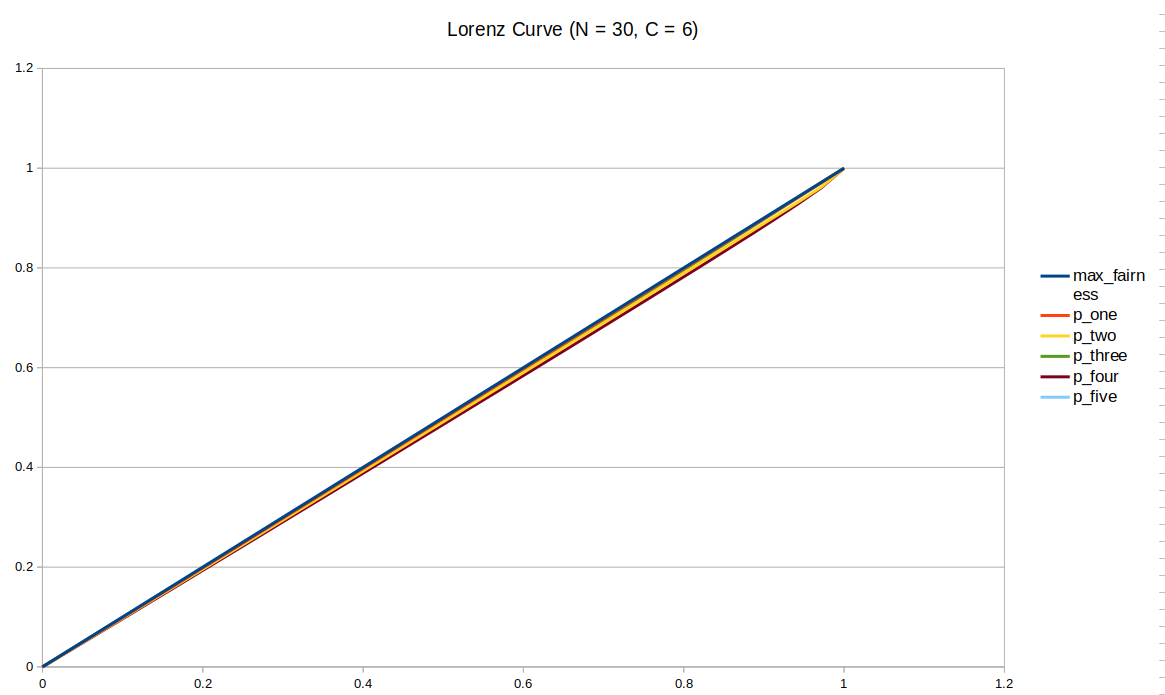
\includegraphics[width=0.9\textwidth]{img/LorenzHighTraffic.png}
%	\caption{Insight 2}
%	\label{img: insight2_respTime}
%\end{figure}
%\begin{figure}[H]
%	\centering
%	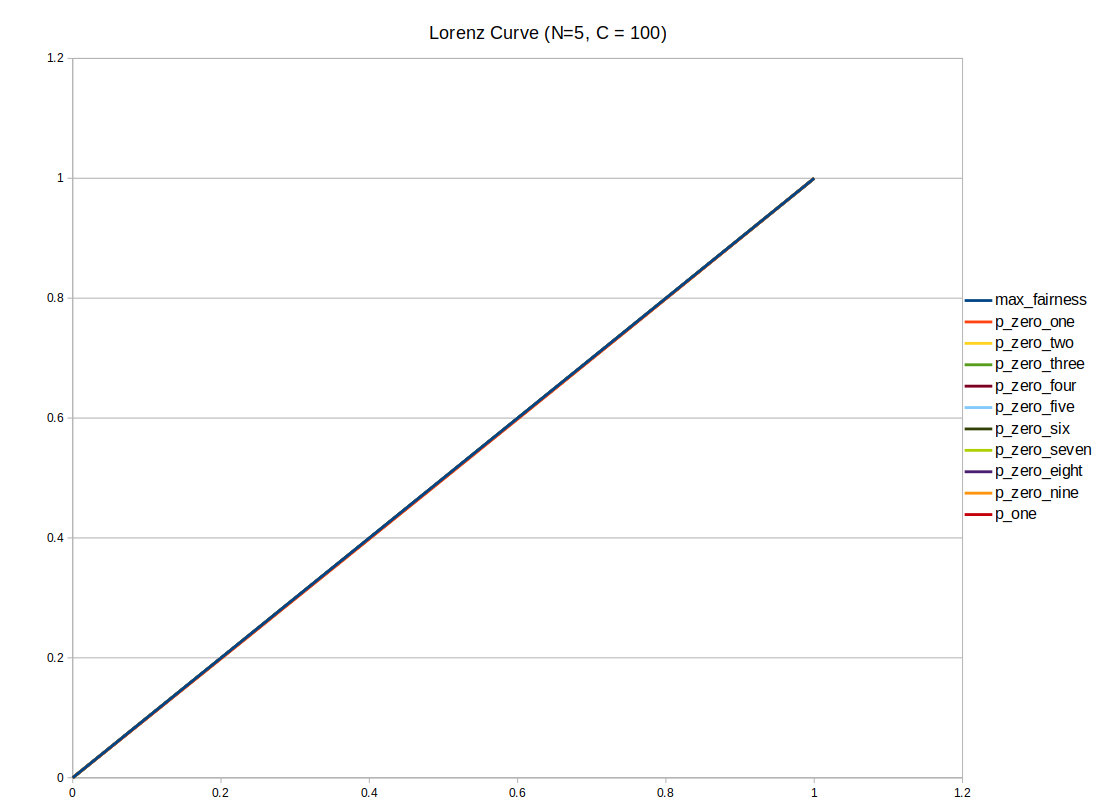
\includegraphics[width=0.9\textwidth]{img/LorenzLowTraffic.png}
%	\caption{Insight 3}
%	\label{img: insight3_respTime}
%\end{figure}

%\noindent \colorbox{yellow}{We can see that in both cases} the curve related to the simulation scenarios are very close to the line of maximum fairness (in the case of low traffic they are overlapping). So we can say that the network protocol is absolutely fair for what regards the response time, whatsoever be the traffic condition.

\subsection{Response Time Explosion Scenario Study}
In this chapter we will study more deeply the case in which we have a \textbf{low mean inter-arrival time} which lead to the "explosion" of the response time. Due to the fact that a \textbf{huge number of collision is expected}, in order to obtain insights for the throughput we created two other \textbf{sub-scenarios} with different behaviour in case of the occurrence of a collision: 
\begin{itemize}
	\item \textbf{(1)} \textit{Change Of Channel in case of collision}: in case of collision of a particular packet, when retrying the retransmission of that packet (after the back-off period) the channel assigned will be picket randomly another time (in general this is the default choice).
	\item \textbf{(2)} \textit{No-Change of Channel in case of collision}
\end{itemize}

We repeated the $2^{k}r$ analysis on the throughput for both sub-scenarios and, \textbf{after verifying the hypothesis} (as we shown before) and \textbf{checking that the $q_{i}$ of the most important factors does non include 0 in the relative 95\% CI scissor}, we obtained the following result:
\begin{itemize}
	\item In both sub-scenarios the number of \textbf{Couples Tx-Rx N} is the \textbf{main factor} in terms of impact on the \textbf{Throughput} (in both cases an impact greater than 50\%)
	\item In both sub-scenarios the number of \textbf{Channels C} has a lower impact on the throughput (around 10\%)
	\item In both sub-scenarios the percentage of the Bernoullian experiment success \textbf{p} had a low impact (4-5\%) on the \textbf{Throughput}
	\item With respect of the limited response time scenario, the \textbf{mean interarrival time} has a \textbf{low impact on the throughput} (around 4\%) 
\end{itemize}
\subsubsection{$2^kr$ Overall Results}
As a reference, in the following table \ref{tab: 2kr_results_explosion} we can see the results obtained through the $r2^k$ analysis.

\begin{itemize}
	\item Number of Couples Tx-Rx: [5, 30] \textbf{(A)}
	\item Number of Channels C : [6, 100] \textbf{(B)}
	\item Send Probability p: [0.1, 1] \textbf{(C)}
	\item Mean Inter-arrival Time: [25ms, 55ms] \textbf{(D)}    
\end{itemize}

\begin{table}[H]
	\centering
	\begin{tabular}{|c|c|c|c|c|}
		\hline
		\textbf{} & \multicolumn{2}{c|}{\textit{\textbf{Throughput Change}}} & \multicolumn{2}{c|}{\textit{\textbf{Throughput No-Change}}} \\ \hline
		Factors   & qi          & Impact on Variability (\%)          & qi            & Impact on Variability (\%)           \\ \hline
		A    & 1.064	& 55.93\% 	& 1.032 &	53.00\%  \\ \hline
		B    & 0.432 &	9.218\% &	0.464 &	10.71\%  \\ \hline
		C    & 0.308 & 4.684\% & 0.290 &	4.207\%  \\ \hline
		D    & -0.285 &	4.033\% & -0.284 &	4.036\%  \\ \hline
		AB   & 0.427 & 9.004\% & 0.458 &	10.47\%  \\ \hline
		AC   & 0.177 & 1.551\% & 0.159 &	1.268\%  \\ \hline
		AD   & -0.143 &	1.0225\% & -0.143 & 1.018\%  \\ \hline
		BC   & 0.144 & 1.026\% &	0.162 &	1.309\%  \\ \hline
		BD   & -0.216 &	2.314\% & -0.216 & 2.338\%  \\ \hline
		CD   & -0.260 & 3.345\% & -0.260 & 3.372\%  \\ \hline
		ABC  & 0.149 & 	1.099\% & 0.167 & 1.397\%  \\ \hline
		ABD  & -0.211 &	2.210\% & -0.211 & 2.230\%  \\ \hline
		ACD  & -0.129 &	0.830\% & -0.129 & 0.834\%  \\ \hline
		BCD  & -0.191 &	1.817\% & -0.192 & 1.847\%  \\ \hline
		ABCD & -0.196 &	1.912\% & -0.197 & 1.945\%  \\ \hline
	
	\end{tabular}
	\caption{Results of $2^k$ analysis for Throughput.}
	\label{tab: 2kr_results_explosion}
\end{table}

\subsection{Response Time Explosion Scenario: Result Analysis}
Due to the fact that the $2^{k}r$ analysis underlined the importance of the Number of Couples Tx-Rx (\textbf{N}) this factor will be taken into consideration for further analysis. The number of Channels and the mean inter-arrival time, from now on, are set to constant due to their limited impact: C=6 and $\frac{1}{\lambda}$ = 35ms. \\
In the following plot we can see more clearly the effects of changing N: the \textbf{throughput increase by increasing N}.
 
\begin{figure}[H]
	\centering
	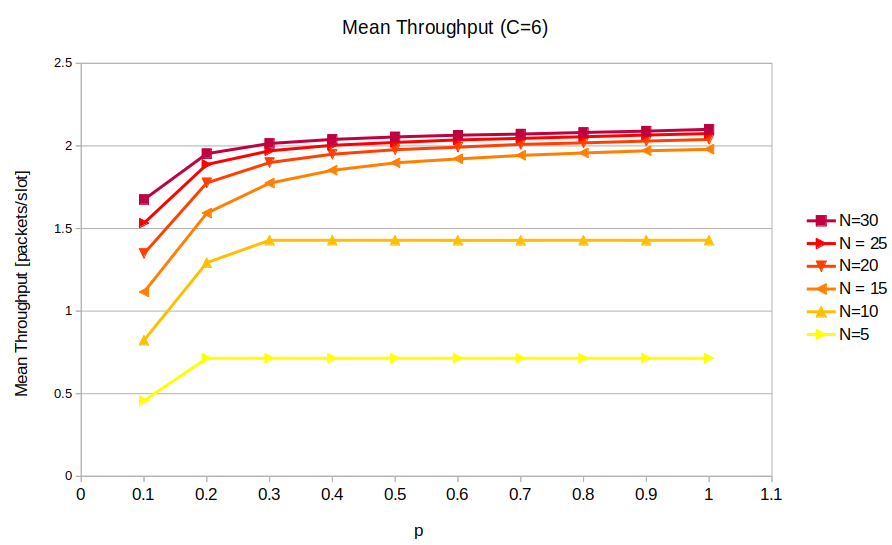
\includegraphics[width=0.8\textwidth]{img/MeanThroughputBufferExplosion.png}
	\caption{Mean Throughput with variation of N and p}
	\label{img: insight4}
\end{figure}

The plot was also done with respect to different values of \textbf{p}, even if such factor does not have a really big impact. This was done because, thinking about the real world, the parameter \textbf{p} is the simplest thing to change, so, even if his impact is not huge, can be a good idea to show which values of p tunes the \textbf{throughput}. All things considered: \textbf{increasing p increases slighly the throughput}, however this increase becomes "smaller" with bigger values of p.\\
For what concerns the \textbf{comparison between the Change Channel sub-scenario with the No-Change one}, the following plot can describe well the differences:
\begin{figure}[H]
	\centering
	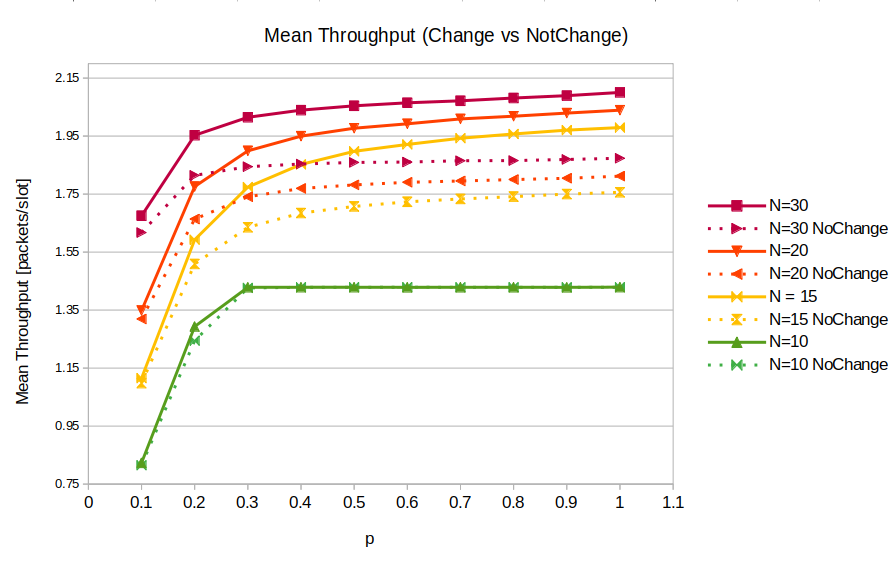
\includegraphics[width=0.8\textwidth]{img/MeanThroughputBufferExplosionChangeVSNoChange.png}
	\caption{Mean Throughput with variation of N and p with different sub-scenarios}
	\label{img: insight3_respTime}
\end{figure}
As we can notice, the dotted lines and the continuous lines represent the same simulation in terms of number N, but with different option of Changing or not the channel in case of collision. So, we can see clearly that for more higher number of N, there is a consistent difference between the two scenarios: \textbf{the sub-scenario without change of the channel is worst in terms of throughput}.